\documentclass{standalone}
\usepackage{tikz}
\usetikzlibrary{positioning}

\begin{document}
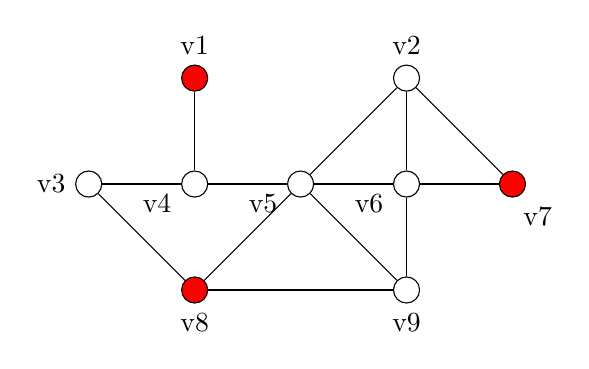
\begin{tikzpicture}
    \node[circle, draw, label=left:v3] (v3) {}; 
    \node[circle, draw, label=185:v4, right = of v3] (v4) {}; 
    \node[circle, draw, label=185:v5, right = of v4] (v5) {}; 
    \node[circle, draw, label=185:v6, right = of v5] (v6) {}; 
    \node[circle, fill=red, draw, label=275:v7, right = of v6] (v7) {}; 
    \node[circle, fill=red, draw, label=v1, above = of v4] (v1) {}; 
    \node[circle, draw, label=v2, above = of v6] (v2) {}; 
    \node[circle, fill=red, draw, label=below:v8, below = of v4] (v8) {}; 
    \node[circle, draw, label=below:v9, below = of v6] (v9) {}; 

    \draw (v1) -- (v4);
    \draw (v2) -- (v6);
    \draw (v6) -- (v9);
    \draw (v3) -- (v4);
    \draw (v4) -- (v5);
    \draw (v5) -- (v6);
    \draw (v6) -- (v7);
    \draw (v3) -- (v8);
    \draw (v8) -- (v5);
    \draw (v5) -- (v2);
    \draw (v2) -- (v7);
    \draw (v5) -- (v9);
    \draw (v8) -- (v9);
\end{tikzpicture}
\end{document}
